% Springer Nature manuscript draft for SIMC NYC.
% Manuscript draft generated from local SIMC_project evidence files.

\documentclass[pdflatex,sn-mathphys-num]{sn-jnl}

\IfFileExists{glyphtounicode.tex}{\input{glyphtounicode}}{}
\pdfgentounicode=1
\usepackage{cmap}
\usepackage[T1]{fontenc}
\usepackage{lmodern}
\usepackage{graphicx}
\usepackage{multirow}
\usepackage{amsmath,amssymb,amsfonts}
\usepackage{booktabs}
\usepackage{tabularx}
\usepackage{array}
\usepackage{adjustbox}
\usepackage{xcolor}
\usepackage{placeins}

\geometry{bindingoffset=0mm,hcentering}
\flushbottom
\setlength{\textfloatsep}{5pt plus 1pt minus 2pt}
\setlength{\floatsep}{5pt plus 1pt minus 2pt}
\setlength{\intextsep}{5pt plus 1pt minus 2pt}
\setlength{\abovecaptionskip}{3pt}
\setlength{\belowcaptionskip}{2pt}
\renewcommand{\arraystretch}{0.92}
\renewcommand{\bibfont}{\footnotesize}
\setlength{\bibsep}{2pt plus 0.3pt}
\hyphenation{calendar category categories categorical component components}
\AtBeginDocument{\hypersetup{allcolors=black, linkbordercolor=black, citebordercolor=black, urlbordercolor=black, filebordercolor=black, pdfborder={0 0 0}}}
\makeatletter
\renewcommand{\email}[1]{\global\advance\emailcnt by 1\relax%
\if@corauemail%
   \g@addto@macro\corrauthemail{\setcounter{footnote}{0}\href{mailto:#1}{\textcolor{black}{#1}};\ }%
\else%
   \g@addto@macro\authemail{\setcounter{footnote}{0}\href{mailto:#1}{\textcolor{black}{#1}};\ }%
\fi}
\makeatother

\begin{document}

\title[Explainable Early Warning for Reported 311 Demand]{Explainable Early Warning for Next-Week Abnormal Reported 311 Demand}

\author*[1]{\fnm{Tran Dai Phong} \sur{Lam}}\email{phonglam2599@gmail.com}
\author[1]{\fnm{Thu} \sur{Le}}\email{thulvm@fpt.edu.vn}
\author[1]{\fnm{Nguyen Quoc} \sur{Hung}}\email{hungtvt2222@gmail.com}
\author[1]{\fnm{Nguyen Trung} \sur{Trinh}}\email{trinhnguyen112355@gmail.com}

\affil*[1]{\orgname{FPT University}, \orgaddress{\city{Ho Chi Minh City}, \country{Vietnam}}}

\abstract{Urban 311 systems provide large-scale traces of reported municipal demand, but they do not directly measure all underlying service need. We frame NYC 311 modeling as a leakage-controlled early-warning problem: for each neighborhood, feature week, and complaint category, predict whether the next week will exceed its recent local baseline by at least 1.5 standard deviations and at least three requests. The study uses 30.9 million NTA-matched requests to construct a 1.33 million-row modeling panel. The selected no-shortcut LightGBM model excludes the 8-week statistics used to construct the target, uses only information available by the end of week \(t\), applies Platt calibration on validation year 2024, and evaluates unchanged on held-out test year 2025. On 2025 test rows, the model obtains PR-AUC 0.317, F1 0.361, precision 0.263, recall 0.574, precision@1\% 0.570, precision@5\% 0.418, and Brier score 0.087; cluster-bootstrap 95\% intervals are reported for the main metrics. Count-forecasting baselines and sparse-target diagnostics show that the task is substantially harder than simple count extrapolation. SHAP beeswarm and local TP/FP/FN waterfall explanations are computed on the LightGBM raw-margin scale before Platt calibration, showing that shifted historical demand dominates while service category, current count, calendar, weather, and borough features refine the alert ranking.}

\keywords{urban computing, 311 service requests, early warning, reported demand, explainable machine learning, calibration, SHAP}

\maketitle

\section{Introduction}\label{sec:introduction}

Urban service agencies increasingly use administrative and resident-generated records to monitor demand and prioritize attention. NYC 311 is a rich example because it records millions of requests across housing, noise, infrastructure, sanitation, water, environmental, and public-safety domains. These records are not a complete census of urban conditions. They mix actual conditions with reporting access, trust, awareness, service expectations, and administrative processing \cite{Wang2017Structure311,KontokostaHong2021Bias}. A forecasting model built on 311 data should therefore be described as forecasting abnormal reported demand, not all underlying need.

We study an operational early-warning task: after feature week \(t\) closes, estimate whether a neighborhood and complaint category will experience an abnormal reported-demand event in week \(t+1\). The model is intended to rank cases for analyst review, not to automate service allocation. This framing makes three design choices central. First, the target should reduce sparse-panel artifacts, where one new request in a historically zero cell can otherwise become a nominal ``surge.'' Second, the feature matrix should not include variables that directly reconstruct the target threshold. Third, evaluation should emphasize ranking, calibration, uncertainty, workload, and error severity, not only a single F1 score.

The contributions are empirical and methodological rather than a claim of a new algorithm. We provide a reproducible NYC 311 neighborhood-week-category panel, define a minimum-count abnormal reported-demand target, compare count and classification baselines, evaluate rolling-origin and held-out future performance, quantify uncertainty and seed stability, calibrate the score layer, audit workload heterogeneity, and explain the actual fitted score model with global and local SHAP outputs.

\section{Related Work}\label{sec:related}

Urban computing connects administrative, geographic, and sensed data to city-scale decision support \cite{Zheng2014UrbanComputing}. Spatiotemporal learning surveys emphasize temporal validation, spatial structure, and careful operational framing in urban prediction problems \cite{Jin2024STGNNSurvey}. Within 311 research, complaint volumes have been used to characterize urban locations \cite{Wang2017Structure311}, but reporting bias can distort data-driven governance decisions \cite{KontokostaHong2021Bias}. Domain studies connect 311 signals to flooding \cite{Agonafir2022Flooding311}, extreme heat \cite{KianmehrPamukcu2022Heat311}, and municipal service design \cite{LiuGarg2024SLA}. Our setting differs by evaluating next-week abnormal reported demand across all neighborhoods and complaint categories in a single chronological panel.

The target is rare and imbalanced, so accuracy is not a useful headline metric. Imbalance-learning and evaluation work motivates reporting precision, recall, F1, PR-AUC, ROC-AUC, and precision at operational review budgets \cite{HeGarcia2009Imbalanced,Fawcett2006ROC,DavisGoadrich2006PRROC,SaitoRehmsmeier2015PR}. Gradient-boosted tree models such as LightGBM are strong tabular baselines for nonlinear interactions \cite{Ke2017LightGBM}. Because alerting systems require transparency, we use TreeSHAP to explain fitted LightGBM score contributions while avoiding causal interpretation of post-hoc explanations \cite{LundbergLee2017SHAP,Lundberg2020TreeSHAP,Rudin2019InterpretableML}.

\section{Methodology}\label{sec:method}

\subsection{Panel and Target}\label{subsec:panel_target}

Source data are NYC Open Data 311 archives for 2010--2019 and 2020--present \cite{NYC311HistoricalOpenData,NYC311OpenData}, 2020 NTA boundaries \cite{NYCNTA2020}, and NOAA GHCN-Daily observations from Central Park station \texttt{GHCND:USW00094728} \cite{Menne2012GHCND}. The analysis window uses 2015--2025 requests spatially joined to 2020 NTAs and aggregated to Monday-start weeks.

Each row corresponds to one NTA \(n\), one feature week \(t\), and one mapped complaint category \(c\). The nine categories are noise, housing, water/sewer, public safety, parking/traffic, environment, infrastructure, sanitation, and other. The deterministic mapping covers 320 original complaint types. Housing, noise, parking/traffic, sanitation, infrastructure, public safety, water/sewer, environment, and other account for 26.06\%, 21.70\%, 21.08\%, 9.99\%, 8.64\%, 5.16\%, 3.92\%, 2.03\%, and 1.43\% of mapped requests, respectively. The full mapping and `other' composition are included in the reviewer-facing supplementary PDF and companion CSV files. The dense panel has 262 NTAs, 575 weekly periods, and nine categories, or 1,355,850 rows. Relative to this dense panel, 30,654 rows are excluded because of warm-up/history requirements and unavailable next-week targets, leaving 1,325,196 model-ready rows (Table \ref{tab:data_summary}).

\begin{table}[!htbp]
\caption{Dataset construction summary.}\label{tab:data_summary}
\centering
\begin{tabular}{@{}llll@{}}
\toprule
Item & Value & Item & Value \\
\midrule
NTA-matched 311 requests & 30,940,129 & Match rate & 99.9777\% \\
Analytical unit & NTA-week-category & Panel rows & 1,355,850 \\
Model-ready rows & 1,325,196 & Excluded rows & 30,654 \\
NTAs & 262 & Complaint categories & 9 \\
Feature weeks & 575 & NOAA station days & 4,018 \\
Final raw predictors & 57 & Encoded model columns & 69 \\
\bottomrule
\end{tabular}
\end{table}

The reference abnormal event is \(\text{count}_{n,t+1,c}>\mu^{8w}_{n,t,c}+1.5\sigma^{8w}_{n,t,c}\), where the mean and standard deviation are computed from a shifted historical eight-week window ending before the target week. To reduce one-call artifacts in near-zero cells, the final target further requires \(\text{count}_{n,t+1,c}\geq3\):
\[
y_{n,t,c}=\mathbf{1}\{\text{count}_{n,t+1,c}>\mu^{8w}_{n,t,c}+1.5\sigma^{8w}_{n,t,c}\ \wedge\ \text{count}_{n,t+1,c}\ge3\}.
\]
The 8-week mean, standard deviation, sum, and ratio used in this target construction are not used as model predictors. Across the 2024--2025 two-year diagnostic period, the T2 target yields 27,277 positives among 247,590 rows and reduces the share of positives from cells with \(\mu^{8w}<1\) from 17.96\% under the original target to 5.10\%.

\subsection{Models and Evaluation}\label{subsec:models_eval}

The final model uses shifted 311 history, current feature-week count, ratios to non-target 12-week history, calendar variables, feature-week weather, service category, and borough identifiers. Weather is a city-level observed exposure for week \(t\); it is not a forecast of week \(t+1\). Contemporary built-environment snapshots are not used in the final model.

The main classifier is LightGBM with the same no-shortcut feature design across folds. The fitted configuration uses 800 trees, learning rate 0.03, 31 leaves, depth 6, minimum child size 100, subsampling and column sampling 0.85, and L2 regularization 3.0. Its training weight is the inverse training prevalence (\texttt{scale\_pos\_weight}); it addresses imbalance during fitting but does not set the alert threshold. The historical hyperparameter grid ranked candidates by validation F1, whereas the revision freeze selects the target and feature scope from validation/rolling-origin PR-AUC, capacity metrics, construct validity, and the documented tie-breakers. A threshold maximizing validation-year F1 is applied unchanged to 2025. Platt calibration was frozen as the final parametric calibrator before held-out reporting; isotonic calibration is retained as a validation-fit sensitivity comparator. The held-out 2025 evaluation trains through 2023, validates on 2024, and tests on 2025. We also report expanding-window folds ending in 2019--2023 with test years 2021--2025, five seeds (42, 123, 2026, 3407, and 7777), and 1,000 NTA-category cluster-bootstrap resamples for the final model. Poisson GLMs use train-fit scaling and train-only categorical encoding; HGB Poisson and hurdle baselines use 260 boosting iterations, learning rate 0.05, 31 leaves, and L2 regularization 0.1. The analyses were run with Python 3.12.10, LightGBM 4.6.0, scikit-learn 1.9.0, pandas 2.3.3, and NumPy 2.3.5. The seed-42 LightGBM fit used for explainability trains in 20.1 seconds on the local workstation; this is a reproducibility diagnostic, not a staffing or deployment latency estimate.

Metrics include PR-AUC, F1, precision, recall, precision@1\%, precision@5\%, Brier score, log loss, expected calibration error (ECE), and alert rate. Precision@k is reported because agencies can review only a fraction of scored rows. Thresholds are fit on validation only. The resulting alerts should be interpreted as a ranking and triage signal rather than an automatic allocation rule.

\section{Results}\label{sec:results}

\subsection{Target, Calibration, and Uncertainty}\label{subsec:main_results}

Table \ref{tab:main_metrics} summarizes the held-out 2025 evidence for the selected no-shortcut LightGBM model. The Platt-calibrated score improves calibration sharply while preserving the ranking metrics, as expected for a monotone score transformation.

\begin{table*}[!htbp]
\caption{Held-out 2025 performance for the selected no-shortcut LightGBM model. Confidence intervals are cluster-bootstrap 95\% intervals over NTA-category clusters.}\label{tab:main_metrics}
\centering
\begin{tabular}{@{}lcc@{}}
\toprule
Metric & Estimate & 95\% CI or stability \\
\midrule
PR-AUC & 0.317 & [0.308, 0.325] \\
F1 & 0.361 & [0.355, 0.368] \\
Precision & 0.263 & [0.258, 0.269] \\
Recall & 0.574 & [0.564, 0.585] \\
Precision@1\% & 0.570 & [0.543, 0.602] \\
Precision@5\% & 0.418 & [0.404, 0.432] \\
Lift@1\% & 5.151 & [4.893, 5.460] \\
Brier score & 0.087 & [0.085, 0.089] \\
Log loss & 0.293 & [0.288, 0.299] \\
Five-seed PR-AUC & 0.319 & SD 0.002 \\
Five-seed F1 & 0.364 & SD 0.002 \\
\bottomrule
\end{tabular}
\end{table*}

Across five rolling-origin folds, the T2 target has mean PR-AUC 0.300, precision@5\% 0.402, and F1 0.358. PR-AUC was 0.308 in 2024 and 0.317 in 2025, while precision@5\% increased from 0.408 to 0.418. Performance was broadly similar across the two most recent folds, although year-specific monitoring remains necessary. In the held-out 2025 evaluation, Platt calibration reduces Brier score from 0.168 to 0.087 and ECE from 0.249 to 0.006. Figure \ref{fig:reliability} shows the resulting reliability curve.

\begin{figure}[!htbp]
\centering
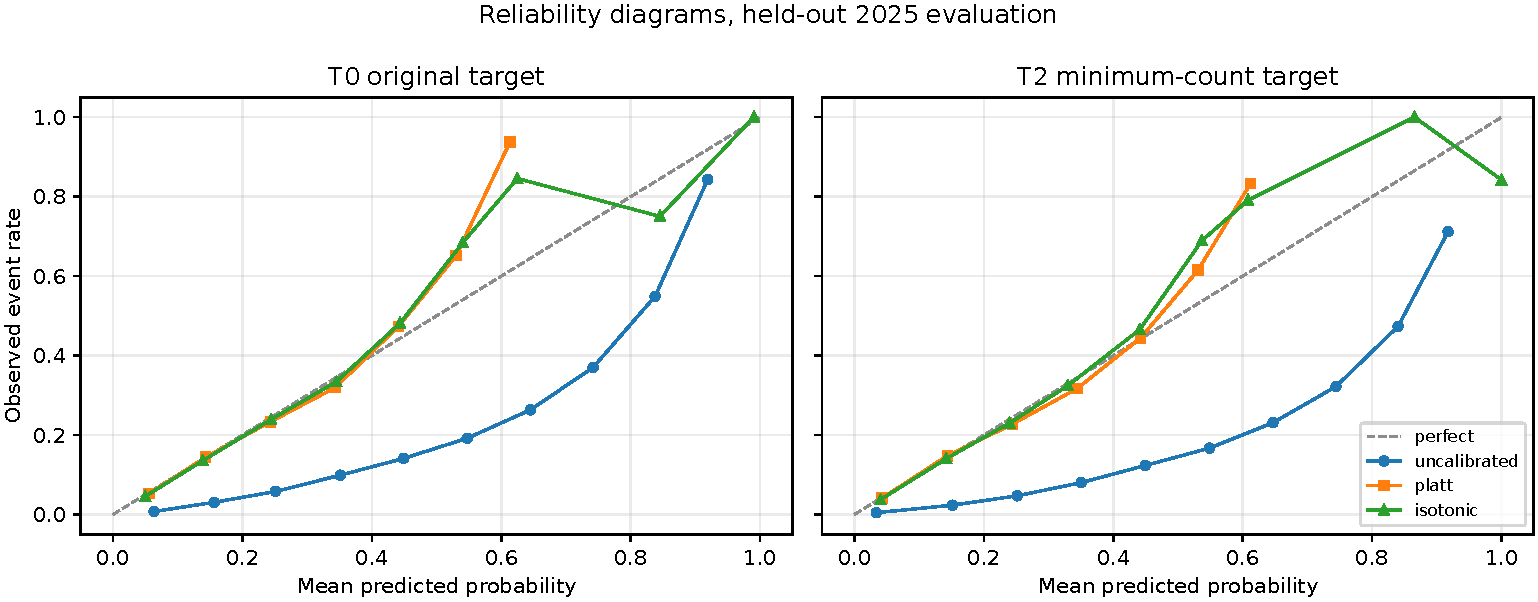
\includegraphics[width=0.78\linewidth]{figures/reliability_diagram.pdf}
\caption{Reliability diagrams for the original T0 target (left) and the final minimum-count T2 target (right). Platt and isotonic calibration are fitted on 2024 validation data and evaluated on held-out 2025 data. T2 is used for the final model.}
\label{fig:reliability}
\end{figure}

\subsection{Baselines and Ablation}\label{subsec:ablation}

Count-model baselines are substantially weaker event rankers than the classification model on the shared T2 task (Table \ref{tab:baselines}). They remain useful as a sanity check: the classifier is not merely reproducing a count forecast with a threshold. A paired NTA-category bootstrap comparing the final LightGBM with the HGB Poisson count baseline gives PR-AUC difference 0.164 [0.156, 0.172] and precision@5\% difference 0.243 [0.227, 0.258]; against the hurdle count baseline, the corresponding differences are 0.165 [0.156, 0.173] and 0.246 [0.230, 0.261]. Supplementary Sections S1--S5 provide volume-decile, mapping, bootstrap, seed, rolling-origin, calibration, and target-sensitivity evidence.

\begin{table*}[!htbp]
\caption{Same-target baseline comparison on held-out 2025 data (122,616 rows; 13,562 T2 positives). Every row is evaluated on the final T2 event. Formula-threshold count decisions apply the T2 abnormal-event rule to predicted counts; the LightGBM threshold is selected on validation 2024.}\label{tab:baselines}
\centering
\begin{adjustbox}{max width=\textwidth}
\begin{tabular}{@{}llrrrrrr@{}}
\toprule
Method & Decision & Count MAE & PR-AUC & P@5\% & Precision & Recall & F1 \\
\midrule
Poisson GLM, no NTA FE & Formula threshold & 9.069 & 0.141 & 0.146 & 0.376 & 0.038 & 0.068 \\
Poisson GLM + NTA fixed effects & Formula threshold & 9.070 & 0.141 & 0.146 & 0.375 & 0.038 & 0.068 \\
HGB Poisson count & T2 formula threshold & 8.021 & 0.153 & 0.176 & 0.513 & 0.103 & 0.171 \\
Hurdle HGB count & T2 formula threshold & 7.938 & 0.152 & 0.172 & 0.497 & 0.111 & 0.181 \\
No-shortcut LightGBM classifier & Validation threshold & -- & 0.317 & 0.418 & 0.263 & 0.574 & 0.361 \\
\bottomrule
\end{tabular}
\end{adjustbox}
\end{table*}

Full-row ablations show that history and current count provide most of the signal, while calendar and weather add smaller increments (Table \ref{tab:ablation}). Weather did not improve validation PR-AUC over history plus calendar in the isolated ablation, although validation precision@5\% and F1 increased slightly. It is retained as a documented contextual covariate and is not treated as a core source of ranking performance. In a five-seed rerun of the key ablation rows, the final borough model has mean test PR-AUC 0.319 (SD 0.002) and the NTA-indicator variant has 0.319 (SD 0.001), so the gain from NTA indicators remains too small to change the simpler final-model claim.

\begin{table*}[!htbp]
\caption{Full-training ablation for the T2 no-shortcut target. Selection uses validation metrics; 2025 test metrics are diagnostic.}\label{tab:ablation}
\centering
\begin{adjustbox}{max width=\textwidth}
\begin{tabular}{@{}lrrrrrr@{}}
\toprule
Feature configuration & Val PR-AUC & Val P@5\% & Val F1 & Test PR-AUC & Test P@5\% & Test F1 \\
\midrule
History lags only & 0.185 & 0.235 & 0.262 & 0.186 & 0.238 & 0.267 \\
History + current count & 0.246 & 0.329 & 0.315 & 0.253 & 0.338 & 0.317 \\
History + calendar & 0.275 & 0.363 & 0.344 & 0.286 & 0.380 & 0.345 \\
History + calendar + weather & 0.274 & 0.364 & 0.347 & 0.295 & 0.389 & 0.354 \\
Final + borough & 0.294 & 0.391 & 0.361 & 0.317 & 0.418 & 0.361 \\
Final + NTA indicators & 0.295 & 0.392 & 0.362 & 0.319 & 0.422 & 0.363 \\
\bottomrule
\end{tabular}
\end{adjustbox}
\end{table*}

\subsection{Workload, Groups, and Error Severity}\label{subsec:workload}

At the validation-selected Platt threshold, the 2025 test year produces a mean of 568.6 alerts per week, with a median of 510 and a range of 97 to 1,055. This volume is high for manual review, so precision@1\% and precision@5\% are more operationally meaningful than F1 alone. Borough alert rates range from 0.209 in Manhattan to 0.259 in Brooklyn; borough precision ranges from 0.245 in Staten Island to 0.308 in Manhattan.

Complaint categories differ sharply (Table \ref{tab:category_metrics}). Noise has the highest alert rate and strongest category F1, while sanitation and other remain weaker. These differences are descriptive performance diagnostics, not a socioeconomic fairness audit. ACS/Census demographic variables are not included, so the reported group diagnostics do not constitute a socioeconomic fairness audit.

\begin{table*}[!htbp]
\caption{Held-out 2025 calibrated LightGBM metrics by complaint category.}\label{tab:category_metrics}
\centering
\begin{adjustbox}{max width=\textwidth}
\begin{tabular}{@{}lrrrrrr@{}}
\toprule
Category & Event prevalence & Alert rate & Precision & Recall & F1 & PR-AUC \\
\midrule
Noise & 0.132 & 0.344 & 0.292 & 0.760 & 0.421 & 0.413 \\
Water/sewer & 0.109 & 0.238 & 0.278 & 0.607 & 0.381 & 0.364 \\
Public safety & 0.109 & 0.232 & 0.282 & 0.598 & 0.384 & 0.300 \\
Housing & 0.122 & 0.214 & 0.295 & 0.519 & 0.376 & 0.382 \\
Parking/traffic & 0.123 & 0.268 & 0.260 & 0.567 & 0.357 & 0.303 \\
Infrastructure & 0.124 & 0.277 & 0.247 & 0.553 & 0.342 & 0.260 \\
Environment & 0.091 & 0.239 & 0.230 & 0.604 & 0.333 & 0.275 \\
Other & 0.090 & 0.153 & 0.253 & 0.431 & 0.319 & 0.260 \\
Sanitation & 0.096 & 0.205 & 0.218 & 0.468 & 0.298 & 0.234 \\
\bottomrule
\end{tabular}
\end{adjustbox}
\end{table*}

Error-severity analysis shows that the final T2 model recalls 57.4\% of positives overall. Recall increases with realized severity: 50.4\% for 1.5--2 standard-deviation exceedances, 56.5\% for 2--3 standard deviations, and 64.4\% for exceedances of at least 3 standard deviations. False negatives therefore still occur in severe events and must be discussed as an operational risk.

\subsection{Explainability}\label{subsec:explainability}

SHAP is computed for the same fitted no-shortcut LightGBM score model used in the held-out 2025 evaluation. It is not an ensemble proxy and it is not a causal explanation. TreeSHAP values are computed on the LightGBM raw-margin scale before Platt calibration. Platt scaling is monotonic for the audited score range and therefore preserves score ordering, but waterfall values and uncalibrated LightGBM probabilities should not be interpreted as calibrated probabilities. The beeswarm in Figure \ref{fig:shap_beeswarm} shows both direction and dispersion of feature effects. Shifted history dominates the global explanation with 72.6\% of summed mean absolute SHAP importance, followed by service category (7.3\%), current count (7.2\%), feature-week weather (6.3\%), calendar (5.5\%), and borough (1.1\%). The weather share reflects citywide feature-week exposure and seasonal correlation in reported demand, not neighborhood microclimate or a forecast of next week's weather. The highest-ranked individual predictors are \texttt{rolling\_12w\_mean}, \texttt{ratio\_to\_12w\_mean}, \texttt{rolling\_4w\_std}, \texttt{complaint\_count}, and \texttt{rolling\_12w\_std}. The formula-aligned 8-week target-construction fields do not appear as predictors.

\begin{figure*}[!htbp]
\centering
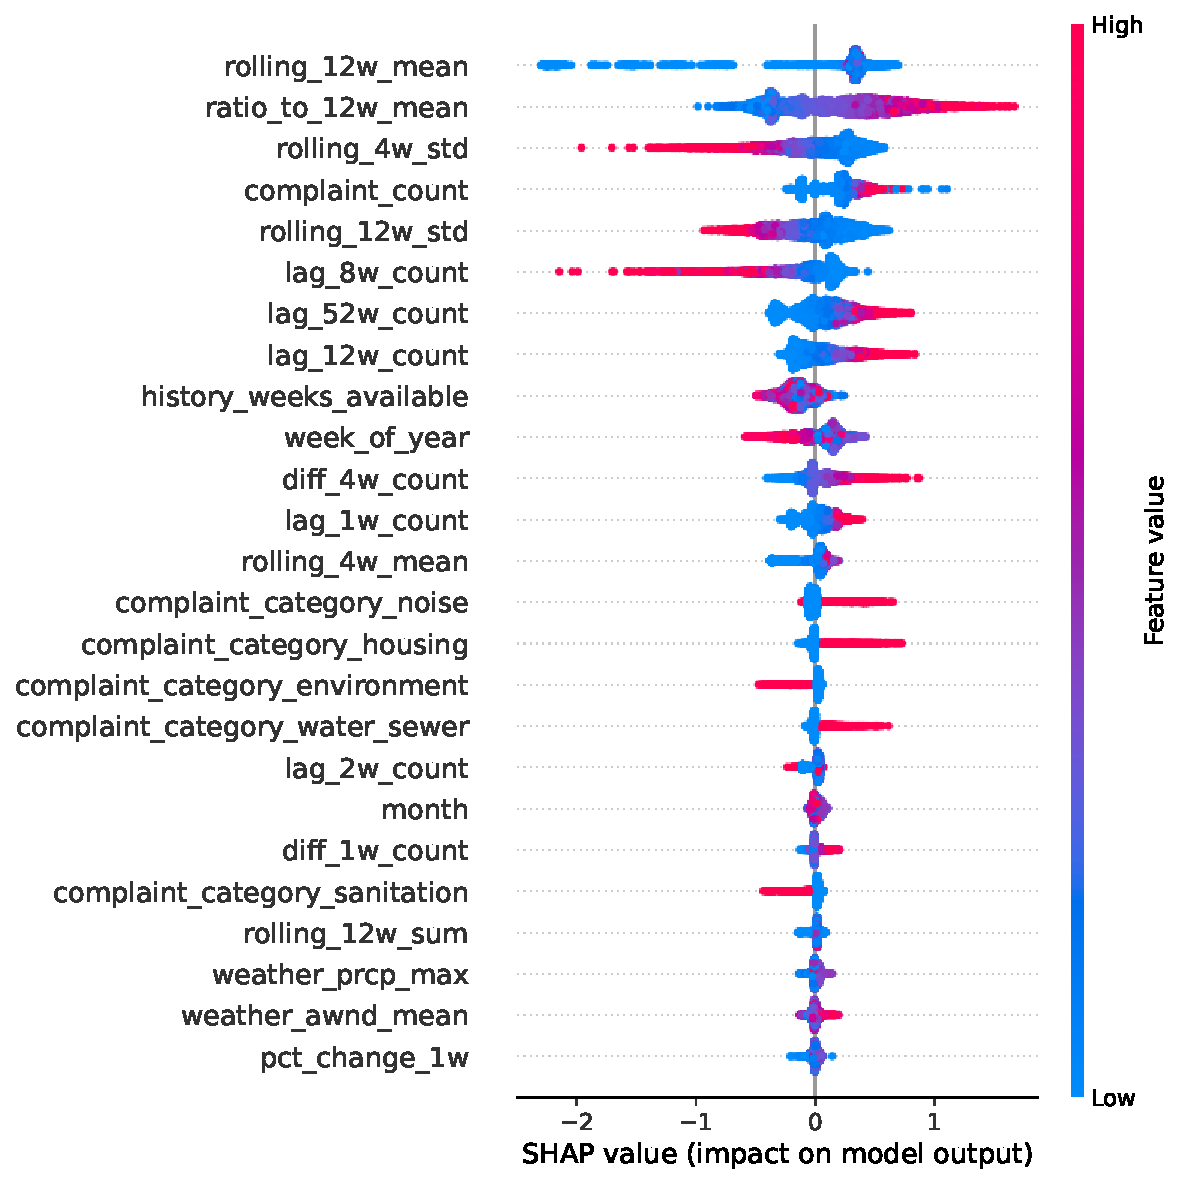
\includegraphics[width=0.95\textwidth]{figures/shap_beeswarm_final.pdf}
\caption{SHAP beeswarm for the selected no-shortcut LightGBM score model on a stratified sample of 8,000 held-out 2025 rows. The explanation model and score model are the same fitted LightGBM; SHAP values are on the pre-calibration raw-margin scale.}
\label{fig:shap_beeswarm}
\end{figure*}

Local cases were selected before interpretation: the highest-probability true positive, the highest-probability false positive, and the missed positive with the largest realized z-exceedance. The Platt-calibrated alert threshold is 0.167. The TP is a Parkchester/Bronx housing case on 2025-10-20 with uncalibrated LightGBM probability 0.975, calibrated probability 0.625, and 244 next-week requests. The FP is a Mapleton-Midwood/Brooklyn noise case on 2025-03-17 with uncalibrated probability 0.956 and calibrated probability 0.603 but no abnormal event. The FN is an Elmhurst/Queens other-category case on 2025-06-30 with uncalibrated probability 0.316, calibrated probability 0.061, and 426 next-week requests, illustrating that large rare shocks can be missed when recent history and category patterns do not support a high pre-event probability.

\begin{figure*}[!htbp]
\centering
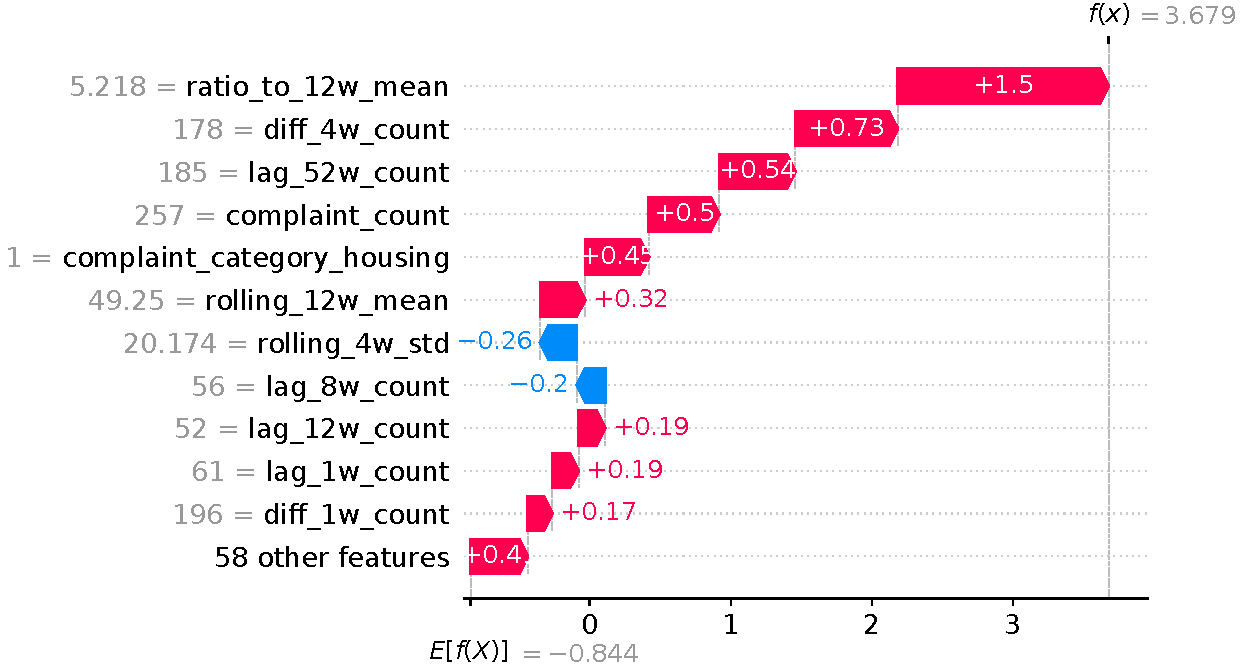
\includegraphics[width=0.90\textwidth]{figures/shap_local_tp.pdf}
\caption{Local SHAP waterfall explanation for the pre-specified high-confidence true-positive case. The waterfall decomposes the LightGBM raw margin before Platt calibration and should not be interpreted as a decomposition of the calibrated probability or as causal attribution.}
\label{fig:local_shap_tp}
\end{figure*}

\begin{figure*}[!htbp]
\centering
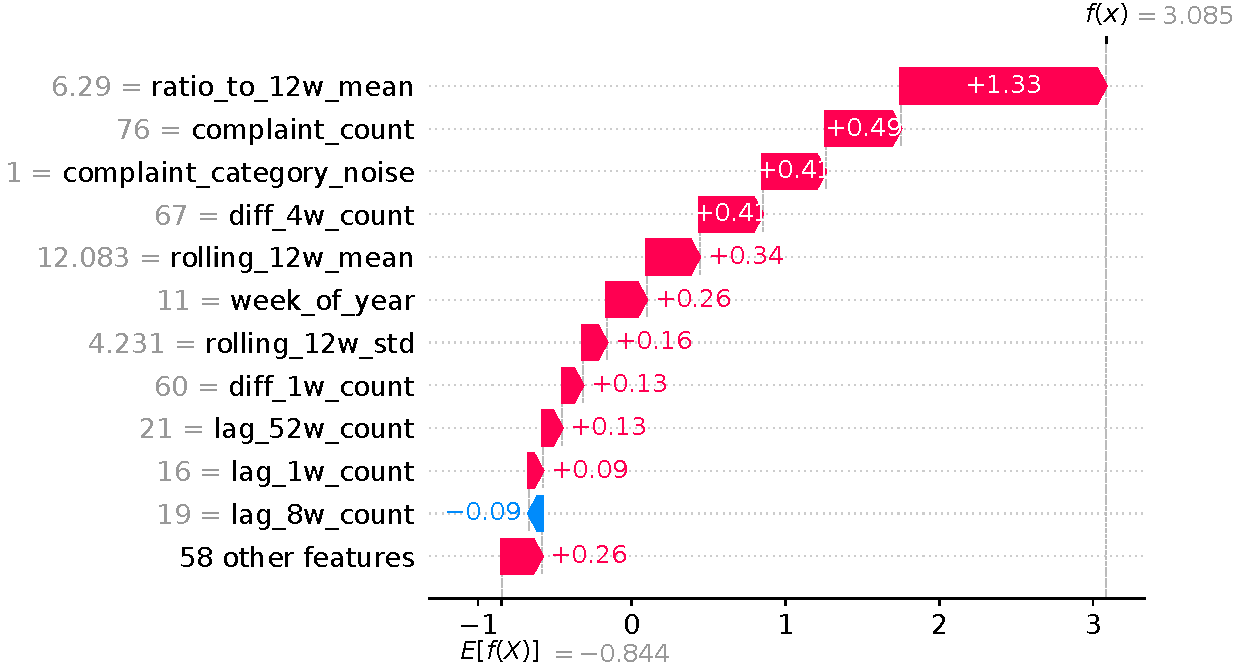
\includegraphics[width=0.90\textwidth]{figures/shap_local_fp.pdf}
\caption{Local SHAP waterfall explanation for the pre-specified high-confidence false-positive case. The waterfall decomposes the LightGBM raw margin before Platt calibration and should not be interpreted as a decomposition of the calibrated probability or as causal attribution.}
\label{fig:local_shap_fp}
\end{figure*}

\begin{figure*}[!htbp]
\centering
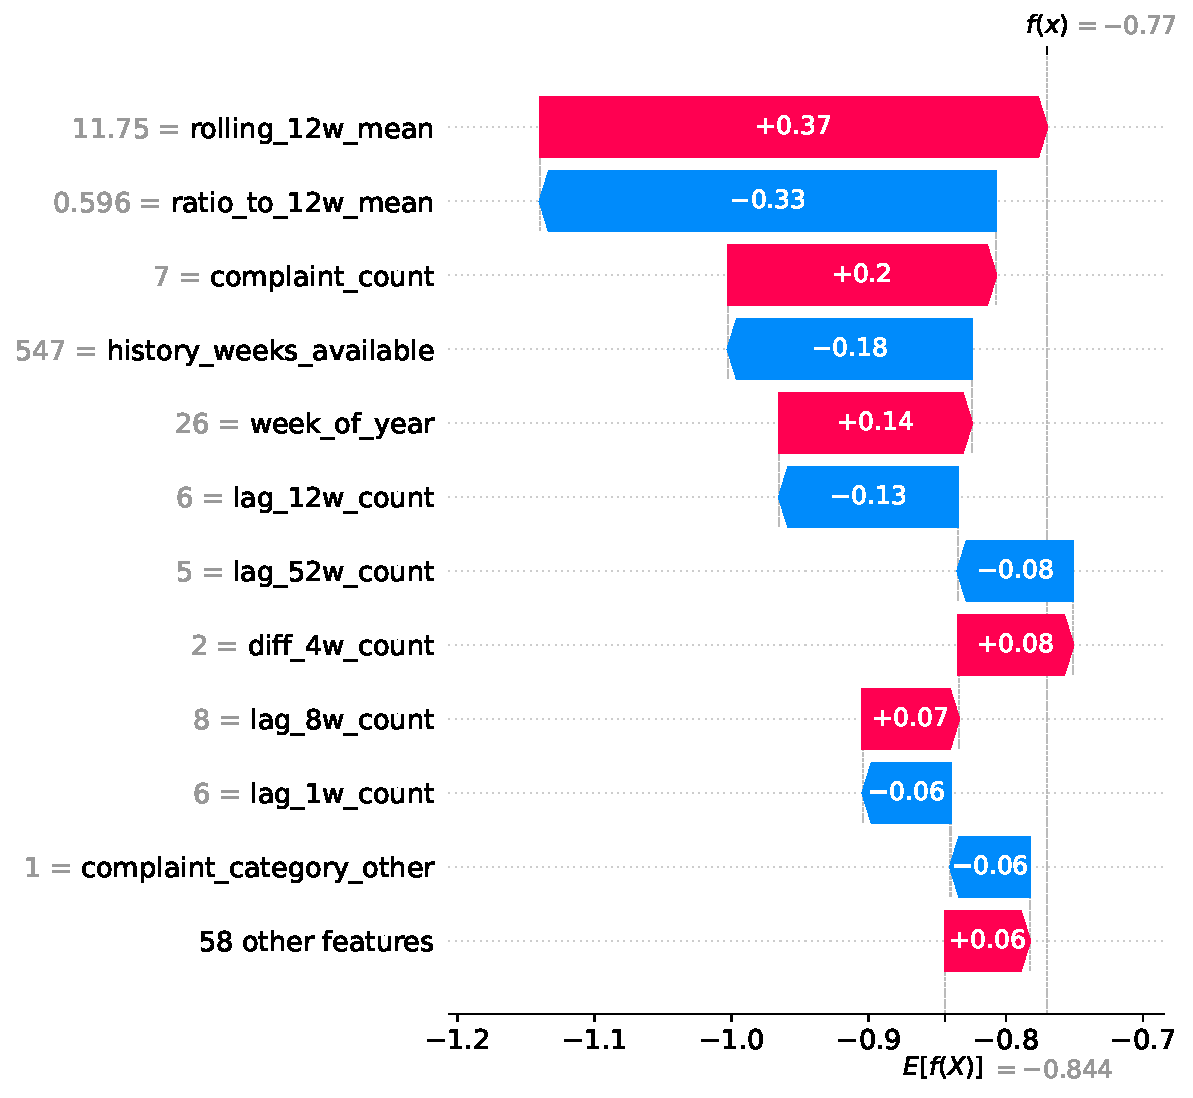
\includegraphics[width=0.90\textwidth]{figures/shap_local_fn.pdf}
\caption{Local SHAP waterfall explanation for the pre-specified severe false-negative case. The waterfall decomposes the LightGBM raw margin before Platt calibration and should not be interpreted as a decomposition of the calibrated probability or as causal attribution.}
\label{fig:local_shap_fn}
\end{figure*}

\FloatBarrier

\section{Discussion}\label{sec:discussion}

The evidence supports a focused claim: the model ranks next-week abnormal reported-demand events more effectively than the evaluated count baselines and history-only configurations, but it should be viewed as a triage aid rather than an automated allocation system. Precision remains modest at the validation-selected alert threshold, while precision@1\% and precision@5\% show stronger concentration when analyst capacity is limited. Any deployment could also create feedback: alerts may change agency attention, resident reporting behavior, and future labels, so prospective monitoring after deployment would be required.

The target redesign improves construct validity in sparse panel cells. Under the original threshold, nearly 18\% of diagnostic-period positives came from cells with \(\mu^{8w}<1\); the T2 target reduces this to 5.10\% by requiring at least three next-week requests. This change also narrows the paper's claim: the task is not raw demand forecasting but early warning for abnormal reported-demand events with a minimum count. A COVID/archive-boundary sensitivity check found visible 2020--2021 prevalence and category-mix shifts; excluding 2020--2021 from training changed 2025 PR-AUC from 0.317 to 0.314 and precision@5\% from 0.418 to 0.412, so the retained training window is treated as a documented sensitivity rather than a homogeneous time series.

Several limitations remain. 311 data reflect reported demand and can reproduce spatial and social reporting inequities. Weather is city-level observed exposure for week \(t\), not a spatial forecast for week \(t+1\). Historical source vintages are unavailable, the modeling panel does not retain row-level archive-source identifiers, and weekly counts may be affected by late entry, reclassification, deduplication, or open-data updates. We therefore cannot fully measure production-time data delay or archive-boundary provenance from the modeling panel. New demographic, staffing, cost, and operational outcome variables are outside the data scope, so socioeconomic fairness, cost-sensitive thresholds, and downstream service impact remain future work. The gain from NTA indicators is small and should be treated as suggestive rather than definitive.

\section{Conclusion}\label{sec:conclusion}

We present a leakage-controlled early-warning study for next-week abnormal reported NYC 311 demand. The final model uses a minimum-count target, removes target-construction shortcut predictors, evaluates chronologically, calibrates probabilities on validation only, and reports uncertainty, seed stability, workload, and local explanations. On held-out 2025 rows, the Platt-calibrated no-shortcut LightGBM model reaches PR-AUC 0.317, F1 0.361, recall 0.574, precision@1\% 0.570, and precision@5\% 0.418. The strongest practical use is not automatic dispatch, but capacity-aware prioritization of analyst attention toward reported-demand risks that merit review.

\section*{Declarations}

\begingroup
\setlength{\parskip}{1pt}
\noindent\textbf{Data and code availability.} Source data include NYC Open Data 311 archives \texttt{76ig-c548} and \texttt{erm2-nwe9}, 2020 NTA boundaries \texttt{9nt8-h7nd}, and NOAA GHCN-Daily observations from Central Park station \texttt{GHCND:USW00094728}. Scripts, complaint-type mappings, configurations, evaluation code, and compact result outputs are available at \texttt{https://github.com/PhongLam26/SIMC\_NYC}. Large intermediate panels can be rebuilt from the public sources using the repository scripts.\par
\noindent\textbf{Competing interests.} The authors declare no competing interests.\par
\noindent\textbf{Funding.} No specific funding was received.\par
\noindent\textbf{Author contributions.} Tran Dai Phong Lam led data processing, modeling, analysis, and drafting; Thu Le served as academic advisor and supervised the study design, methodology, and manuscript editing; Nguyen Quoc Hung and Nguyen Trung Trinh contributed validation and review.
\endgroup

\setlength{\bibsep}{2pt plus 0.3pt}
\renewcommand{\bibfont}{\footnotesize}
\bibliography{references}

\end{document}
